\documentclass[10pt,a4paper]{beamer}
\usepackage[utf8]{inputenc}
\usepackage{amsmath}
\usepackage{amsfonts}
\usepackage{graphicx}
\usepackage{animate}
\usepackage{physics}
\usepackage{amssymb}
\usepackage{mathrsfs}
\usepackage[utf8]{inputenc}
\usetheme{Warsaw}  %% Themenwahl

%Hamiltonian simulation algorithms for near-term quantum hardware
\title[]{Hamiltonian simulation algorithms for near-term quantum hardware}
\author{Patrick Bettermann}
\date{\today}
\newcommand*\oldmacro{}%
\let\oldmacro\insertshorttitle%
\renewcommand*\insertshorttitle{%
  \oldmacro\hfill%
  \insertframenumber\,/\,\inserttotalframenumber}


\begin{document}
\maketitle
\setbeamertemplate{section in toc}[circle]
\frame{\tableofcontents[]}


\section{Hamiltonian simulation}

\begin{frame} %%Eine Folie
  \frametitle{Problem statement} 
  \begin{Definition} 
  Hamiltonian simulation: \\
  	"Given a description of a Hamiltonian H, and evolution time t, some initial state $\ket{\psi(0)}$  produce the final state $\ket{\psi(t)}$ (to some error $\epsilon$)"
  \end{Definition}
  \begin{itemize}
 	\item "The Hamiltonian of a system is the sum of the kinetic energies of all the particles, plus the potential energy of the particles associated with the system
	\end{itemize}
\end{frame}

            
\subsection{}
\begin{frame}
  \frametitle{Why is this a difficult problem?} 
  	\begin{Definition}
  	We assume that the quantum state is loaded into memory
	\end{Definition}
\vspace{0.3in}
 \begin{itemize}
 	\item a classical computer can't store the state efficiently
 	\item a classical computer cannot produce a complete description of the state
 	\end{itemize}
\end{frame}


\subsection{Schrödinger equation}
\begin{frame}
  \frametitle{Schrödinger equation} 
  \begin{Definition}
  $ H \ket{\psi(t)} = i \hbar \frac{\delta}{\delta t} \ket{\psi(t)} $
  \end{Definition}
  \vspace{0.21in}
  integrate both sides:\\
  \vspace{0.11in}
  \quad $ \ket{\psi(t)} = e^{-iHt/\hbar} \ket{\psi(0)}$\\
  \vspace{0.11in}
  break H down into potential and kinetic energy: \\
  \quad $\hat{V}$ (E_{pot}), E_{kin} = $\frac{p^{2}}{2m}$ \\
  \vspace{0.11in}
  \quad $e^{\frac{-i\hat{V}t}{\hbar}}$ and $e^{\frac{-ip^2t}{2m\hbar}}$ don't commute, 
  $e^{-iHt/\hbar} \neq e^{\frac{-i\hat{V}t}{\hbar}}e^{\frac{-ip^2t}{2m\hbar}}$
\end{frame}



\subsection{Lie-Trotter product formula}
\begin{frame}
  \frametitle{Lie-Trotter product formula}
  \begin{Definition}
  $ e^{A+B} = \lim_{n \to \inf}(e^{A/n}e^{B/n})^{n}  $
  \end{Definition}
  \begin{itemize}
  	\item product formula: simulate the sum-terms of a Hamiltonian by simulating each one separetly for a small time slice
  	\item $ H = A + B + C $
  	\item $ U = e ^ {-i(A+B+C)t} = (e^{-iCt/r}e^{-iBt/r}e^{-iCt/r})^{r} $
  	\item switching between kinetic and potential energy terms
  \end{itemize}
  we arrive at: $e^{\frac{-i\hat{H}t}{\hbar}} =  \lim_{N\to\infty} (e^{\frac{-ip^2t}{2m \hbar N}}e^{\frac{-\hat{V}(\hat{x})t}{\hbar N}})^N$
\end{frame}


\section{Implementation}
\subsection{Split operator}
\begin{frame}

\begin{Definition}
 Split operator
\end{Definition}
  
Algorithm: \\

\begin{enumerate}
\item Apply a half step of the potential propagator to $\psi(0)$ \\
\item Apply the Fourier transform: momentum basis \\
\item Apply a full step of the kinetic propagator on the momentum basis\\
\item Apply the Inverse Fourier transform: back to coordinate basis\\
\item Apply the second half step of the potential propagator\\
\end{enumerate}
\vspace{0.1in}
this algorithm results from splitting the propagator, substituting into the Schrödinger equation and projecting onto a coordinate basis $\ket{x}$
\end{frame}

\subsection{Simulating a wavefunction}
\begin{frame}
  \frametitle{Simulating a wavefunction}
  \begin{itemize}
  	\item blue line:  $\bra{\Psi}\ket{\Psi}$ 
  	\item orange line: potential energy, $\hat{V}$
  \end{itemize}
  \animategraphics[loop,autoplay, width=1\linewidth]{12}{figures/without_well/animation_without_well-}{0}{399}
\end{frame}

\begin{frame}
  \frametitle{Simulating a wavefunction}
  \begin{itemize}
  	\item blue line:  $\bra{\Psi}\ket{\Psi}$ 
  	\item orange line: potential energy, $\hat{V}$
  \end{itemize}
  \animategraphics[loop,autoplay, width=1\linewidth]{12}{figures/with_well/animation_with_well-}{0}{399}
\end{frame}




\section{Hamiltonian simulation algorithms for near-term quantum hardware}
\subsection{Introduction}
\begin{frame}
  \frametitle{Problem statement}
  \begin{Definition}
  Find explicit gate count for near-term simulations
  \end{Definition}
  \begin{itemize}
  	\item gate count of near-term quantum hardware is very limited
  	\item algorithms need to be optimized to use as few gates as possible
  	\item even low gate counts of 250 gates are still too costly
  \end{itemize}    
\end{frame}

\begin{frame}
\frametitle{Topics}
  \begin{itemize}
    \item Optimal fermion encoding 
  	\item Subscircuits: programming below the circuit model
  	\item Non-asymptotic Trotter bounds
  \end{itemize}    
\end{frame}

\subsection{Fermi-Hubbard Model}
\begin{frame}
 \frametitle{Fermi-Hubbard Model}
  Hamiltonian: \\
  $H_{FH} =  \sum_{i=1}^{N} h_{on-site}^{(i)} + \sum_{i<j,\sigma}^{} h_{hopping}^{(i,j,\sigma)}$
  \vspace{0.1in}
  \begin{itemize}
  	\item Model existed before quantum computing
  	\item Most practical applications involve fermionic system
  	\item Classical approaches can be used as benchmark
  \end{itemize}
  
\end{frame}


\subsection{Sub-Circuit Model}
\begin{frame}
 \frametitle{Sub-Circuit Model}
  \begin{itemize}
  	\item Assumption: hardware can perform CNOT, Z, H .... gates
  	\item Layer of abstraction: overhead
  	\item Quantum circuit: $ C = \prod_{l}^{L} U_{l}V_{j} $
  	\item U_{l} = \prod_{i \in Q} u_{i}^{l}$ a layer of arbitrary single qubit unitary gates $
  	\item $V_{l} = \prod_{i j \in \Gamma} v_{i j} (t_{ij}^{l})$ a layer of non-overlapping, two-qubit gates
  	\item two-qubit unitary gates: $v_{ij}(t) = e^{ith_{ij}}, h_{ij} = Z_{i}Z_{j}$
  	\item $h_{ij} = \sigma_{i}\sigma_{j}$ since $ \sigma_{i}\sigma_{j} = Z_{i}Z_{j}$(*)
  	\item the cost $T_{cost}(C) = L$, L = circuit depth 
  \end{itemize}
\end{frame}


\begin{frame}
	\frametitle{Sub-Circuit Synthesis}
    \begin{Definition}
    how to decompse local Trotter steps $e^{i\delta h}$\\
    Let $U(t) = e^{itH}, H = \frac{1}{2i}[h_1, h_2]$\\
    $U(t) = e^{it_1 h_1}e^{it_2 h_2}e^{it_2 h_1}e^{it_1 h_2}$ (Lemma 7, supplementary)
    \end{Definition} 
    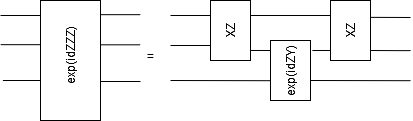
\includegraphics[width=\textwidth,height=0.4\textheight,keepaspectratio]
            {figures/gate_decomp.png}
\end{frame}



\subsection{Trotter bounds}
\begin{frame}
	\frametitle{Error models}
	\begin{enumerate}
		\item Per-gate error model
		\item Per-time error model
	\end{enumerate}
		\vspace{0.11in}
	\begin{itemize}
		\item "Error budget required to execute a circuit"
		\item Single-qubit gates are considered free
		\item Obtain tight error expression $\epsilon_p (\delta)$
		\item Guarantee $\epsilon_p (\delta) < \epsilon_{target}$ by inverting the expression and derive a maximum possible Trotter step $\delta_0 = \delta_0 (\epsilon_{target})$
	\end{itemize}
\end{frame}


\section{Results}
\subsection{Per-gate run-times}
\begin{frame}
	\frametitle{Run-times}
	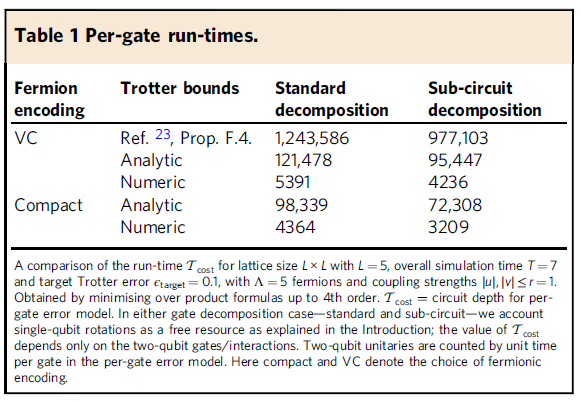
\includegraphics[width=\textwidth,height=0.6\textheight,keepaspectratio]
            {figures/per-gate-run-time.png}
	\linebreak   
	\begin{flushleft}
		source: Hamiltonian simulation algorithms for near-term quantum hardware, Clinton et al.
	\end{flushleft}	 
\end{frame}

\begin{frame}
	\frametitle{Per-time run-times}
	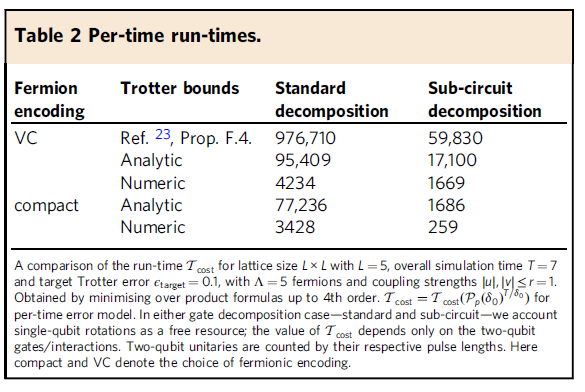
\includegraphics[width=\textwidth,height=0.6\textheight,keepaspectratio]
            {figures/per-time-run-time.png}
	\linebreak   
	\begin{flushleft}
		source: Hamiltonian simulation algorithms for near-term quantum hardware, Clinton et al.
	\end{flushleft}	 
\end{frame}

\subsection{Gate decomposition cost}
\begin{frame}{Outline}
	\frametitle{Gate decomposition cost}
	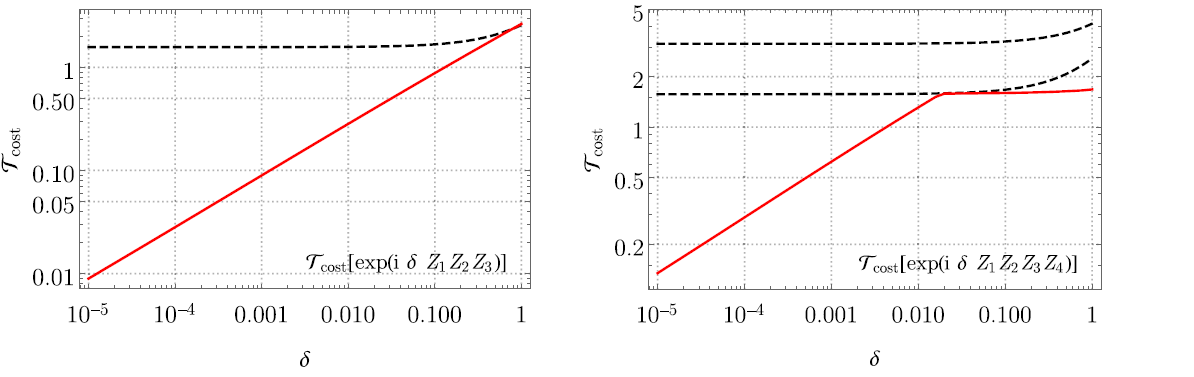
\includegraphics[width=\textwidth,height=0.6\textheight,keepaspectratio]
            {figures/gate-decomposition-cost.png}
    \begin{flushleft}
		source: Hamiltonian simulation algorithms for near-term quantum hardware, Clinton et al.
	\end{flushleft}
\end{frame}

\section{Outlook}
\begin{frame}
\frametitle{Outlook}
\begin{itemize}
	\item Further optimization needed for quantum hardware
	\item Tighter error bounds might be reached
	\item Standard circuit decomposition will stay unfeasible on real hardware for some time
	\item The sub-circuit model might enable some algorithm to run on NISQ hardware
\end{itemize}
\end{frame}

\section{End}
\begin{frame}
\title{End}
	\begin{center}
		Thank you for your attention!
	\end{center}
\end{frame}


\end{document}